\clearpage

{\color{red} 

\section {Updated Analysis Using the Full T2K Run 1-9 Dataset} \label{sec:run1-9d_update}

A statistical update to the Run 1-9c results has been performed with the addition of the Run 9d dataset. The analysis procedure is identical to that of the Run 1-9c analysis, but there has been the following changes to the analysis inputs:

\begin{itemize}
	\item An increase of $\nub$ mode exposure of $\SI{46}{\%}$ from $\TotalPotNuBarRunOneNineC$ POT to $\TotalPotNuBarRunOneNine$ POT
	\item Updated the Gaussian reactor constraint on $\sin^{2} 2 \theta_{13}$ from the 2016 PDG value of $0.0857 \pm 0.0046$ to the 2018 PDG value of $0.0830 \pm 0.0031$, as shown in the updated prior table \ref{tab:osc_param_priors_nuebarapp_Run1-9d}
	\item Updated the Asimov A true value of $\sin^{2} 2 \theta_{13}$ to 0.0830, to match the central value of the above 2018 PDG reactor constraint
	\item An updated flux tuning using an updated version of FLUKA and nuclear interaction model \cite{flux_tuning_Run1-9d}
\end{itemize}

\begin{table}
	\centering
	\begin{tabular}{| c | c | c | c |}
 	\hline
Parameter(s)													& Prior		& Range     												\\
\hline
$\sin^{2}\theta_{23}$											&  Uniform 	& $[0.3; 0.7]$     							 				\\
$\sin^{2} 2 \theta_{13}$ reactors		&  Gaussian & $0.0830 \pm 0.0031$ 										\\
%$\sin^{2} 2 \theta_{13}$ ($\sin^{2} \theta_{13}$) T2K only	   	&  uniform	& $[0; 0.4]$ 	\\
$\sin^{2} 2 \theta_{12}$  										&  Gaussian & $0.846 \pm 0.021$ 										\\
$|\Delta m^{2}_{32}|$ (NH) / $|\Delta m^{2}_{13}|$ (IH)      	&  Uniform	& $ [2.3; 2.7] \times 10^{-3}~\mbox{eV}^2/\mbox{c}^4$	    \\
$\Delta m^{2}_{21}$      										&  Gaussian & $(7.53 \pm 0.18) \times 10^{-5}~\mbox{eV}^2/\mbox{c}^4$	\\
$\delta_{CP}$                                               	&  Uniform 	& $[-\pi; +\pi]$ 											\\
Mass Hierarchy													&  Bernoulli& 0.5 normal, 0.5 inverted 									\\  
\hline
\end{tabular}
\caption{
Treatment of the oscillation parameters in the $\nueb$ appearance analysis. All the gaussian priors are from \cite{pdg_2018}. The parameter $\sin^{2} 2 \theta_{13}$ is constrained with the measurement of reactor experiments using the gaussian prior. The nominal values of $\sin^2 2 \theta_{13}$, $\sin^2 2 \theta_{12}$ and $\Delta m^2_{21}$ are from \cite{pdg_2018}, while all the other oscillation parameter values corresponds to the most probable values obtained by the Bayesian analysis on the T2K run 1-4 neutrino mode data \cite{T2KLongPaper}.
}
\label{tab:osc_param_priors_nuebarapp_Run1-9d}
\end{table}


As part of the validation process two additional studies have been performed: An updated test of the p-value stability (see appendix \ref{app:pval_stability_Run1-9d}), and a comparison of the toy generation methods used by the VALOR and P-theta groups (see appendix \ref{app:sampling_vs_reweighting}).



\subsection{Sensitivity to $\nueb$ Appearance} \label{sec:run1-9d_sensitivity}

The sensitivity study is performed as described for the Run 1-9c analysis (see sec \ref{sec:sensitivity}). The expected event rates for all five Super-K event samples using the updated Asimov A parameters are shown in \Crefrange{tab:event_rates_exp_1Rmu_R1-9d}{tab:event_rates_exp_MultiRe_Run1-9d}. Although there has been no change in the neutrino mode exposure, the event rates in the neutrino mode samples have changed slightly compared to the Run 1-9c values due to the updated flux tuning.

%\documentclass[10pt,a4paper]{article}
%\usepackage[utf8]{inputenc}
%\usepackage{amsmath}
%\usepackage{amsfonts}
%\usepackage{amssymb}
%\usepackage{fullpage}
%\begin{document}
%
%\section*{Job details}
%
%
%\begin{minipage}[t]{0.5\textwidth}
%\begin{itemize}
%\item[] $\sin^2(\theta_{12})$ = 0.304
%\item[] $\sin^2(\theta_{13})$ = 0.0212
%\item[] $\sin^2(\theta_{23})$ = 0.528
%\item[] $\Delta m^2_{21}$ = 7.53e-05
%\item[] $|\Delta m^2_{32}|$ = 0.002509
%\item[] $\delta_{CP}$ = -1.601
%\end{itemize}
%\end{minipage}
%\\
%
%
%
%BANFF tunings: Enabled
%
%Hierarchy: Normal
%
%
%\section*{1Rmu}
\begin{table}
	\centering
	\begin{tabular} { | l ||r | r | r | r | r | r | | r | }
	\hline
	              & $\nu_\mu$            & $\nu_e$              & $\bar{\nu}_{\mu}$    & $\bar{\nu}_{e}$      & Osc. $\nu_e$         & Osc. $\bar{\nu}_{e}$ & Total                \\ \hline\hline
	 CCQE         & 178.45275            & 0.00420              & 11.18602             & 0.00019              & 0.02219              & 0.00014              & 189.66550            \\ \hline
	 CC1pi        & 28.23407             & 0.00203              & 2.65612              & 0.00009              & 0.02380              & 0.00007              & 30.91619             \\ \hline
	 CCcoherent   & 0.29228              & 0.00000              & 0.09292              & 0.00000              & 0.00000              & 0.00000              & 0.38520              \\ \hline
	 2p2h         & 35.80423             & 0.00153              & 1.44684              & 0.00008              & 0.02483              & 0.00004              & 37.27755             \\ \hline
	 CCother      & 5.52439              & 0.00086              & 0.40845              & 0.00008              & 0.00011              & 0.00001              & 5.93389              \\ \hline
	 NC1pi0       & 0.62495              & 0.01869              & 0.02138              & 0.00143              & N/A                  & N/A                  & 0.66646              \\ \hline
	 NC1piPM      & 4.99423              & 0.09960              & 0.17726              & 0.00980              & N/A                  & N/A                  & 5.28090              \\ \hline
	 NCcoherent   & 0.00000              & 0.00000              & 0.00044              & 0.00003              & N/A                  & N/A                  & 0.00048              \\ \hline
	 NCother      & 2.10279              & 0.07529              & 0.13268              & 0.00923              & N/A                  & N/A                  & 2.31998              \\ \hline
	\hline
	 Total        & 256.02970            & 0.20221              & 16.12211             & 0.02094              & 0.07094              & 0.00026              & 272.44616            \\ \hline
	\end{tabular}
	\caption{Predicted number of events in the neutrino mode single-ring $\mu$-like sample obtained after applying the BANFF weight for a total exposure of \TotalPotNuRunOneNine\ FHC POT. The Asimov data set A in Tab \ref{tab:osc_params_joint_asimovA} is used. The total of 272.44616 events consists of 256.02970 signal events and 16.41647 background events.}
\label{tab:event_rates_exp_1Rmu_R1-9d}
\end{table}

%Total: 272.44616    (272.44616)
%
%
%Total signal: 256.02970
%
%
%Total background: 16.41647
%
%POT: 14.93798E20
%
%
%\section*{1Re}
\begin{table}
	\centering
	\begin{tabular} { | l ||r | r | r | r | r | r | | r | }
	\hline
	              & $\nu_\mu$            & $\nu_e$              & $\bar{\nu}_{\mu}$    & $\bar{\nu}_{e}$      & Osc. $\nu_e$         & Osc. $\bar{\nu}_{e}$ & Total                \\ \hline\hline
	 CCQE         & 0.16374              & 6.41338              & 0.00641              & 0.25515              & 45.62597             & 0.27069              & 52.73533             \\ \hline
	 CC1pi        & 0.04802              & 0.95057              & 0.00284              & 0.06769              & 4.44444              & 0.04635              & 5.55993              \\ \hline
	 CCcoherent   & 0.00012              & 0.00842              & 0.00018              & 0.00394              & 0.03387              & 0.00317              & 0.04970              \\ \hline
	 2p2h         & 0.03051              & 1.60651              & 0.00120              & 0.04313              & 8.46160              & 0.03827              & 10.18123             \\ \hline
	 CCother      & 0.01340              & 0.12849              & 0.00034              & 0.00930              & 0.08589              & 0.00313              & 0.24056              \\ \hline
	 NC1pi0       & 1.72930              & 0.03761              & 0.06069              & 0.00357              & N/A                  & N/A                  & 1.83117              \\ \hline
	 NC1piPM      & 0.17178              & 0.00480              & 0.01033              & 0.00057              & N/A                  & N/A                  & 0.18749              \\ \hline
	 NCcoherent   & 0.53883              & 0.00729              & 0.04868              & 0.00296              & N/A                  & N/A                  & 0.59776              \\ \hline
	 NCother      & 0.32454              & 0.01730              & 0.02153              & 0.00129              & N/A                  & N/A                  & 0.36467              \\ \hline
	 NC1gamma     & 0.96236              & 0.01722              & 0.05061              & 0.00235              & N/A                  & N/A                  & 1.03254              \\ \hline
	\hline
	 Total        & 3.98261              & 9.19160              & 0.20281              & 0.38996              & 58.65176             & 0.36161              & 72.78036             \\ \hline
	
	\end{tabular}
	\caption{Predicted number of events in the neutrino mode single-ring e-like sample obtained after applying the BANFF weight for a total exposure of \TotalPotNuRunOneNine\ FHC POT. The Asimov data set A in Tab \ref{tab:osc_params_joint_asimovA} is used. The total of 72.78036 events consists of 58.65176 signal events and 14.12860 background events.}
	\label{tab:event_rates_exp_1Re_Run1-9d}
\end{table}
%
%Total: 72.78036    (72.78036)
%
%
%Total signal: 58.65176
%
%
%Total background: 14.12860
%
%POT: 14.93798E20
%
%
%
%\clearpage
%
%
%\section*{RHC1Rmu}

\begin{table}
	\centering
	\begin{tabular} { | l ||r | r | r | r | r | r | | r | }
	\hline
	              & $\nu_\mu$            & $\nu_e$              & $\bar{\nu}_{\mu}$    & $\bar{\nu}_{e}$      & Osc. $\nu_e$         & Osc. $\bar{\nu}_{e}$ & Total                \\ \hline\hline
	 CCQE         & 33.23334             & 0.00183              & 64.88124             & 0.00199              & 0.00198              & 0.00287              & 98.12326             \\ \hline
	 CC1pi        & 8.61735              & 0.00072              & 9.82622              & 0.00054              & 0.00126              & 0.00129              & 18.44737             \\ \hline
	 CCcoherent   & 0.10172              & 0.00000              & 0.37877              & 0.00010              & 0.00000              & 0.00013              & 0.48073              \\ \hline
	 2p2h         & 9.62489              & 0.00056              & 6.23791              & 0.00058              & 0.00091              & 0.00044              & 15.86529             \\ \hline
	 CCother      & 2.03601              & 0.00025              & 1.28783              & 0.00000              & 0.00000              & 0.00000              & 3.32409              \\ \hline
	 NC1pi0       & 0.13032              & 0.00479              & 0.13243              & 0.00358              & N/A                  & N/A                  & 0.27112              \\ \hline
	 NC1piPM      & 0.78284              & 0.03295              & 0.99469              & 0.02624              & N/A                  & N/A                  & 1.83671              \\ \hline
	 NCcoherent   & 0.00000              & 0.00000              & 0.00439              & 0.00000              & N/A                  & N/A                  & 0.00439              \\ \hline
	 NCother      & 0.69330              & 0.03560              & 0.43187              & 0.01681              & N/A                  & N/A                  & 1.17759              \\ \hline
	\hline
	 Total        & 55.21978             & 0.07670              & 84.17534             & 0.04984              & 0.00416              & 0.00472              & 139.53053            \\ \hline
	
	\end{tabular}
	\caption{Predicted number of events in the antineutrino mode single-ring $\mu$-like sample obtained after applying the BANFF weight for a total exposure of \TotalPotNuBarRunOneNine\ RHC POT. The Asimov data set A in Tab \ref{tab:osc_params_joint_asimovA} is used. The total of 139.53053 events consists of 84.17534 signal events and 55.35520 background events.}
	\label{tab:event_rates_exp_RHC1Rmu_Run1-9d}
\end{table}

%Total: 139.53053    (139.53053)
%
%
%Total signal: 84.17534
%
%
%Total background: 55.35520
%
%POT: 16.34556E20
%
%
%\section*{RHC1Re}

\begin{table}
	\centering
	\begin{tabular} { | l ||r | r | r | r | r | r | | r | }
	\hline
	              & $\nu_\mu$            & $\nu_e$              & $\bar{\nu}_{\mu}$    & $\bar{\nu}_{e}$      & Osc. $\nu_e$         & Osc. $\bar{\nu}_{e}$ & Total                \\ \hline\hline
	 CCQE         & 0.02796              & 1.10898              & 0.05220              & 1.82304              & 2.15856              & 5.96183              & 11.13258             \\ \hline
	 CC1pi        & 0.01660              & 0.21958              & 0.01604              & 0.30984              & 0.30251              & 0.70366              & 1.56823              \\ \hline
	 CCcoherent   & 0.00005              & 0.00214              & 0.00091              & 0.02278              & 0.00240              & 0.06516              & 0.09344              \\ \hline
	 2p2h         & 0.00633              & 0.30850              & 0.00484              & 0.24505              & 0.48467              & 0.69725              & 1.74663              \\ \hline
	 CCother      & 0.00835              & 0.04508              & 0.00253              & 0.02421              & 0.02166              & 0.01383              & 0.11566              \\ \hline
	 NC1pi0       & 0.30059              & 0.01164              & 0.38057              & 0.00988              & N/A                  & N/A                  & 0.70269              \\ \hline
	 NC1piPM      & 0.05384              & 0.00275              & 0.04314              & 0.00171              & N/A                  & N/A                  & 0.10143              \\ \hline
	 NCcoherent   & 0.10435              & 0.00481              & 0.44089              & 0.00678              & N/A                  & N/A                  & 0.55682              \\ \hline
	 NCother      & 0.12374              & 0.00477              & 0.05756              & 0.00212              & N/A                  & N/A                  & 0.18819              \\ \hline
	 NC1gamma     & 0.17384              & 0.00959              & 0.38085              & 0.00822              & N/A                  & N/A                  & 0.57250              \\ \hline
	\hline
	 Total        & 0.81566              & 1.71784              & 1.37954              & 2.45362              & 2.96980              & 7.44172              & 16.77817             \\ \hline
	
	\end{tabular}
	\caption{Predicted number of events in the antineutrino mode single-ring e-like sample obtained after applying the BANFF weight for a total exposure of \TotalPotNuBarRunOneNine\ RHC POT. The Asimov data set A in Tab \ref{tab:osc_params_joint_asimovA} is used. The total of 16.77817 events consists of 7.44172 signal events and 9.33646 background events.}
	\label{tab:event_rates_exp_RHC1Re_Run1-9d}
\end{table}

%Total: 16.77817    (16.77817)
%
%
%Total signal: 7.44172
%
%
%Total background: 9.33646
%
%POT: 16.34556E20
%
%
%
%\clearpage
%
%
%\section*{MultiRe}

\begin{table}
	\centering
	\begin{tabular} { | l ||r | r | r | r | r | r | | r | }
	\hline
	              & $\nu_\mu$            & $\nu_e$              & $\bar{\nu}_{\mu}$    & $\bar{\nu}_{e}$      & Osc. $\nu_e$         & Osc. $\bar{\nu}_{e}$ & Total                \\ \hline\hline
	 CCQE         & 0.02898              & 0.02486              & 0.00118              & 0.00173              & 0.20835              & 0.00258              & 0.26767              \\ \hline
	 CC1pi        & 0.07743              & 0.77592              & 0.00261              & 0.00385              & 4.79666              & 0.00222              & 5.65868              \\ \hline
	 CCcoherent   & 0.00027              & 0.01791              & 0.00008              & 0.00007              & 0.10930              & 0.00010              & 0.12773              \\ \hline
	 2p2h         & 0.01020              & 0.02210              & 0.00050              & 0.00096              & 0.15575              & 0.00103              & 0.19054              \\ \hline
	 CCother      & 0.03776              & 0.11255              & 0.00115              & 0.00275              & 0.11687              & 0.00144              & 0.27253              \\ \hline
	 NC1pi0       & 0.02080              & 0.00077              & 0.00084              & 0.00008              & N/A                  & N/A                  & 0.02249              \\ \hline
	 NC1piPM      & 0.06592              & 0.00167              & 0.00387              & 0.00033              & N/A                  & N/A                  & 0.07179              \\ \hline
	 NCother      & 0.21033              & 0.00847              & 0.01326              & 0.00090              & N/A                  & N/A                  & 0.23296              \\ \hline
	 NC1gamma     & 0.02908              & 0.00000              & 0.00068              & 0.00007              & N/A                  & N/A                  & 0.02983              \\ \hline
	\hline
	 Total        & 0.48077              & 0.96425              & 0.02418              & 0.01074              & 5.38692              & 0.00737              & 6.87423              \\ \hline
	
	\end{tabular}
	\caption{Predicted number of events in the neutrino mode $\nue \textrm{CC}1\pi^{+}$-like sample obtained after applying the BANFF weight for a total exposure of \TotalPotNuRunOneNine\ FHC POT. The Asimov data set A in Tab \ref{tab:osc_params_joint_asimovA} is used. The total of 6.87423 events consists of 5.38692 signal events and 1.48730 background events.}
	\label{tab:event_rates_exp_MultiRe_Run1-9d}
\end{table}

%Total: 6.87423    (6.87423)
%
%
%Total signal: 5.38692
%
%
%Total background: 1.48730
%
%POT: 14.93798E20
%
%\end{document}


The distributions of the event-rate in the antineutrino mode single-ring e-like sample for both hypotheses are shown in Fig \ref{fig:sensitivity_rate-only_Run1-9d} and the $\Delta \chi^2$ distributions for both hypotheses are shown in Fig \ref{fig:sensitivity_rate+shape_Run1-9d}. The corresponding Asimov A p-values are shown in Tab \ref{tab:sensitivity_AsimovA_R1-9d}. A comparison to the sensitivity study produced by the P-theta group is shown in appendix \ref{app:compare_sensitivity_valor_ptheta}.

\begin{table}
	\centering
	\begin{tabular}{|c|c|c|c|c|}
		\hline
		$\beta$				& Analysis		& p-value                		& $\sigma$ 						    & Asimov A Test Statistic\\
		\hline
		\multirow{ 2}{*}{0} & rate-only		& \pvalRateOnlyBetaZeroAsimovARunOneNineD  & \sigmaRateOnlyBetaZeroAsimovARunOneNineD    & \multirow{ 2}{*}{N.A.}    \\
		\cline{2-4}
			   				& rate+shape	& \pvalRateShapeBetaZeroAsimovARunOneNineD & \sigmaRateShapeBetaZeroAsimovARunOneNineD   &    \\
		\hline
		\multirow{ 2}{*}{1} & rate-only		& \pvalRateOnlyBetaOneAsimovARunOneNineD   & \sigmaRateOnlyBetaOneAsimovARunOneNineD     & $N_{events} = \NskOscExpectationNueBarRunOneNineD \pm \NskOscExpectationNueBarErrorRunOneNineD$ (syst) \\
		\cline{2-5}
			   				& rate+shape	& \pvalRateShapeBetaOneAsimovARunOneNineD  & \sigmaRateShapeBetaOneAsimovARunOneNineD    & $\Delta \chi^2 = \DeltachisqAsimovARunOneNineD$ \\
		\hline
	\end{tabular}
	\caption{Asimov A p-values and event-rates for the $\beta = 0$ and $\beta = 1$ hypotheses using both the rate-only and rate+shape analyses and the full Run 1 - 9 dataset. There are no Asimov A expectations for the $\beta = 0$ hypothesis, as the Asimov A dataset assumes that $\beta = 1$ is true.}
	\label{tab:sensitivity_AsimovA_R1-9d}
\end{table}


For both rate-only and rate+shape analyses, the Asimov A sensitivity using the full Run 1-9 dataset gives a $\sim \SI{0.3}{\sigma}$ stronger exclusion of the $\beta=0$ hypothesis compared to the sensitivity using the Run 1-9c dataset. There is approximately no change in the exclusion of the $\beta=1$ hypothesis. A more detailed comparison of the full Run 1-9 results to the Run 1-9c results can be found in appendix \ref{app:compare_R1-9d_R1-9c}.


\begin{figure}
	\centering
	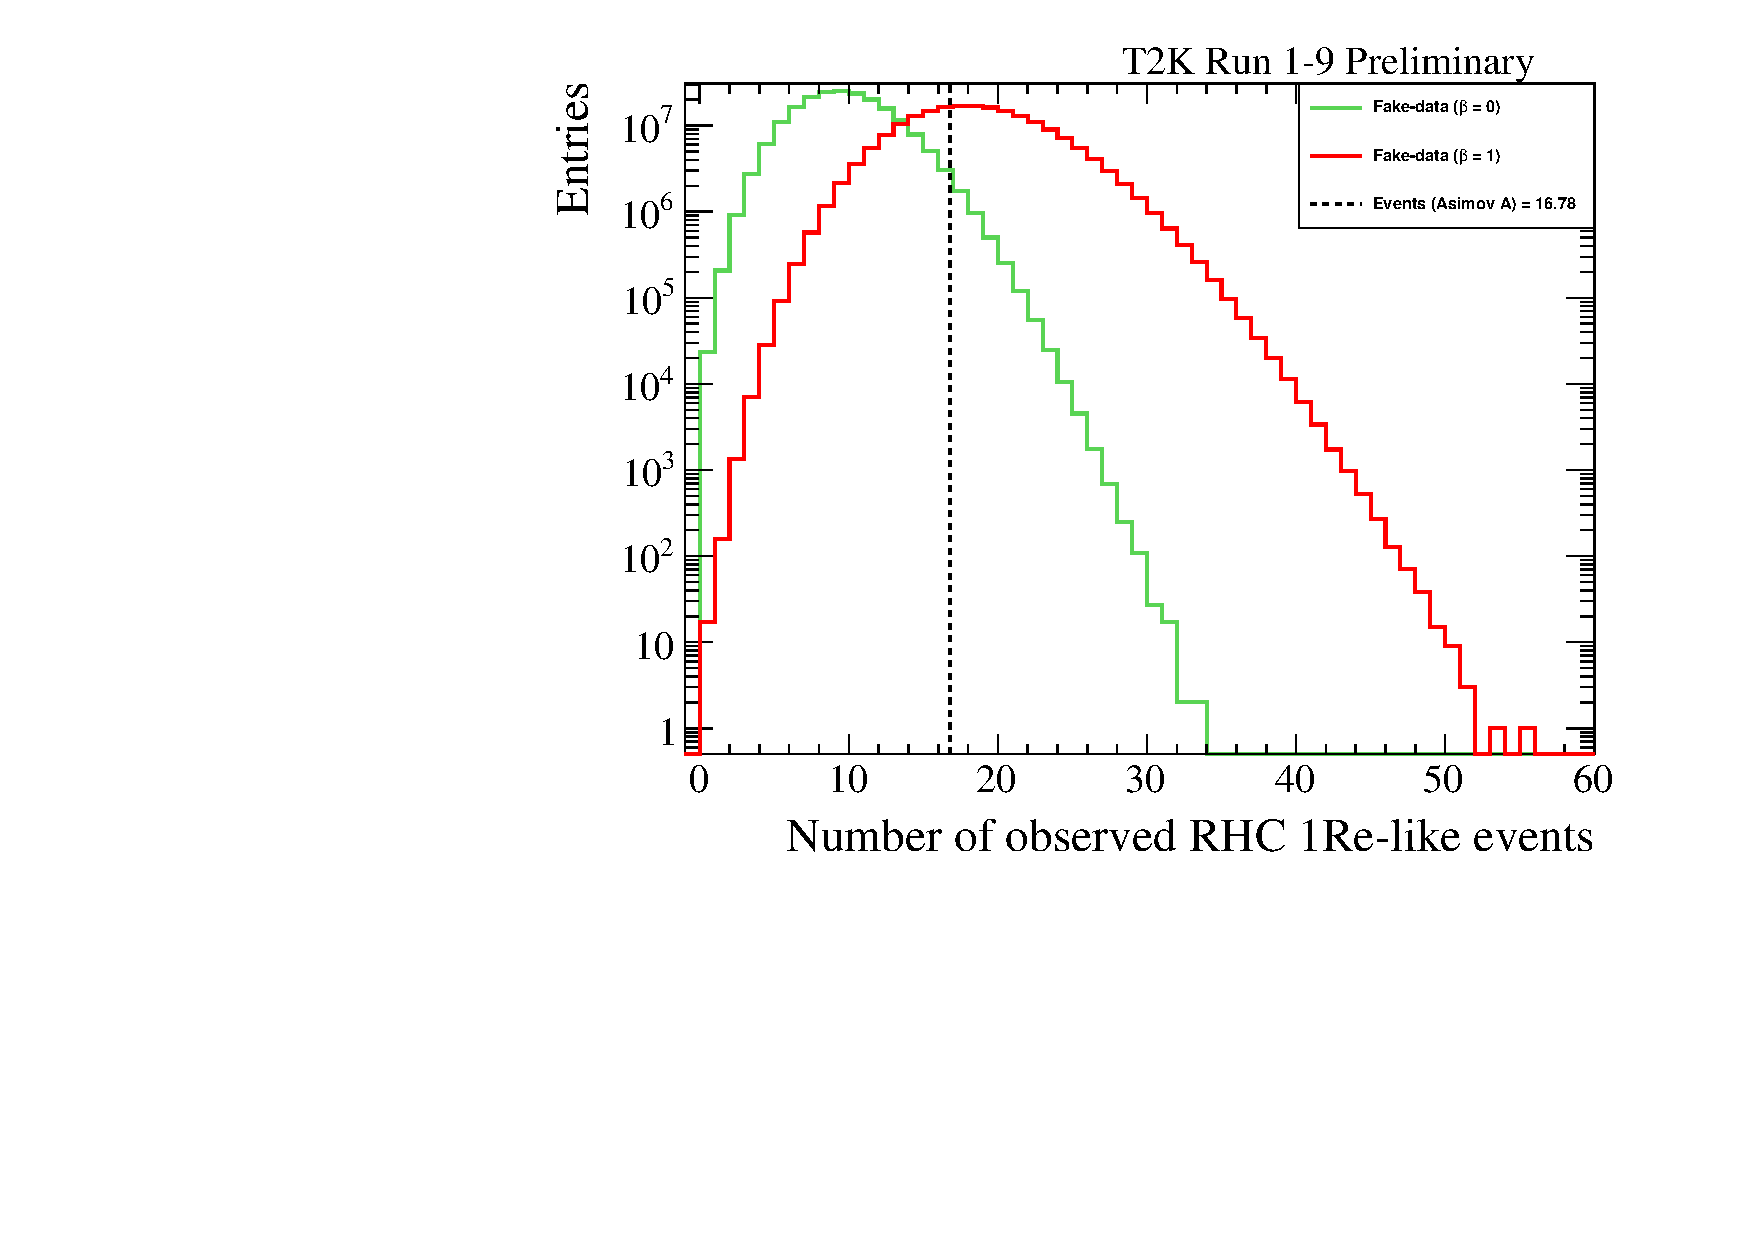
\includegraphics[scale=0.65]{sensitivity/plots_Run1-9d/sensitivity_weighted_2019-01-18/nuebarapp_graphs_nmargtoys_200k_nexp_20k_rate-only_MCsampling_PDG2018_VALOR_Nevents_logscale}
	\caption{The distribution of the total number of events in the antineutrino mode single-ring e-like sample from each of the \NToysFakeDataRateOnly\ toy experiments for both the $\beta = 0$ and $\beta = 1$ hypotheses using full Run 1 - 9 statistics. The distributions were produced using the method outlined in section \ref{sec:method_rate-only} using the Asimov A spectra to calculate the 4-sample likelihood. The dashed line corresponds to the total number of events given by the Asimov A data set.}
	\label{fig:sensitivity_rate-only_Run1-9d}
\end{figure}

\begin{figure}
	\centering
	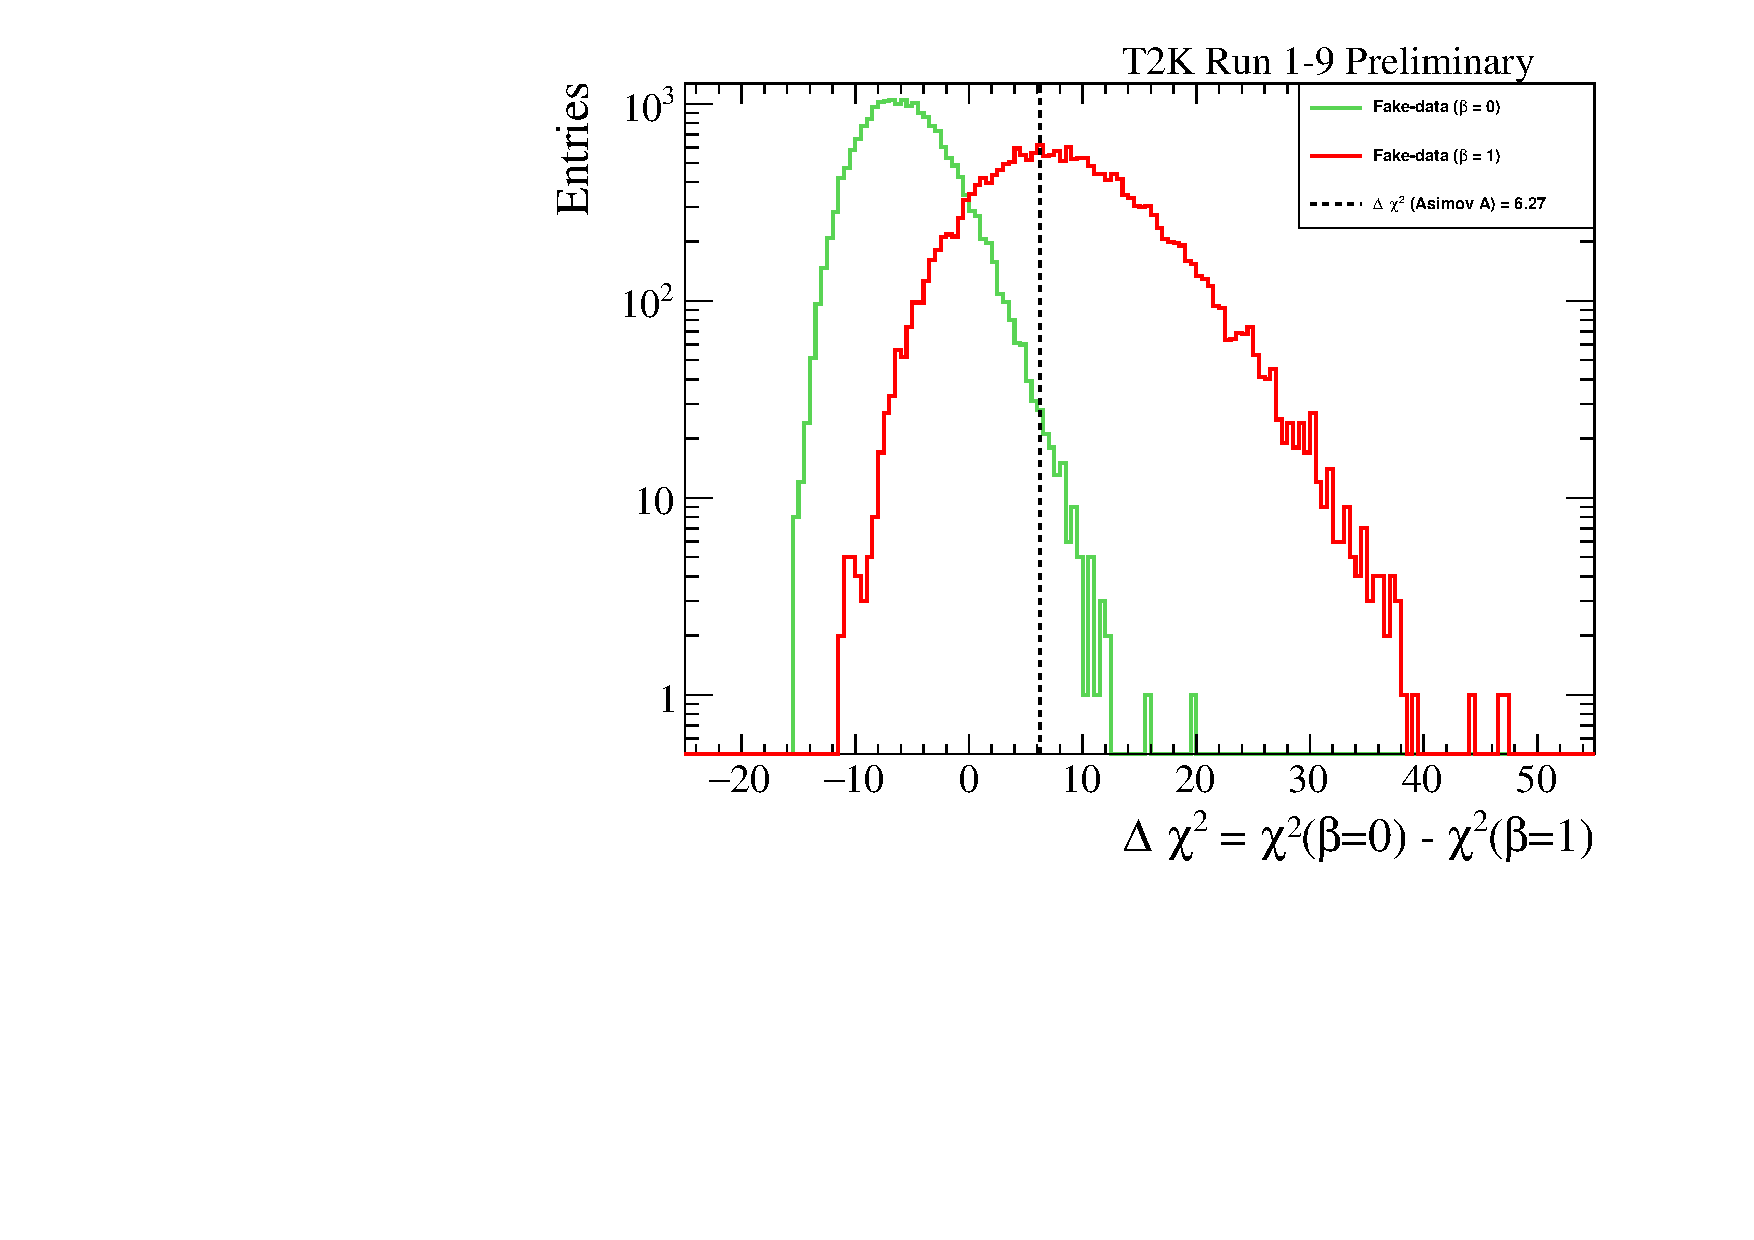
\includegraphics[scale=0.65]{sensitivity/plots_Run1-9d/sensitivity_weighted_2019-01-18/nuebarapp_graphs_nmargtoys_200k_nexp_20k_rate+shape_MCsampling_PDG2018_VALOR_Deltachisq_logscale}
	\caption{The distribution of $\Delta \chi^2$ values from each of the \NToysFakeDataRatePlusShape\ toy experiments for both the $\beta = 0$ and $\beta = 1$ hypotheses using full Run 1 - 9 statistics. The distributions were produced using the method outlined in section \ref{sec:method_rate+shape} using the Asimov A spectra to calculate the 4-sample likelihood. The dashed line corresponds to the $\Delta \chi^2$ value given by the Asimov A data set.}
	\label{fig:sensitivity_rate+shape_Run1-9d}
\end{figure}



\FloatBarrier

\subsection{Results of the $\nueb$ Appearance Analysis} \label{sec:run1-9d_results}

The rate-only and rate+shape p-values for $\nueb$ appearance are performed on the full Run 1-9 data set following the same procedure as in Sec \ref{sec:method}. 1-sided p-values are computed on the right tail of the test statistic expected distribution to exclude $\beta = 0$ and the left tail to exclude $\beta = 1$. Fig \ref{fig:asimova_spectra_all_Run1-9d} shows the data in the 5 Super-K event samples overlaid with the expected event rates for Asimov data set A. In Figs \ref{fig:data_rate-only_Run1-9d} and \ref{fig:data_rate+shape_Run1-9d} the distributions of the test statistic, for rate-only and rate+shape analyses, are shown and compared with the data. The  observed number of events in the antineutrino mode single-ring e-like sample in Super-K was \NskObservedNueBarRunOneNineD. The observed $\Delta \chi^2$ value was \DeltachisqDataRunOneNineD. The p-values resulting from these distributions and test statistic values are shown in Tab \ref{tab:data_pvals_R1-9d}. A comparison to observed p-values produced by the P-theta group is shown in appendix \ref{app:compare_data_valor_ptheta}..

As shown in Tab \ref{tab:data_pvals_R1-9d}, both the rate-only and rate+shape analyses disfavour the $\beta = 0$ hypothesis more than the $\beta = 1$ hypothesis. The Jeffreys scale indicates that the Bayes factor (see eq. \ref{eq:bayes_factor}) of \BayesFactorDataRunOneNineD\ corresponds to a substantial preference for the $\beta = 1$ hypothesis over $\beta = 0$. This preference is in contrast to the earlier Run 1-9c and Run 1-7 analyses, which both had a poor preference for the $\beta = 0$ hypothesis over $\beta = 1$. The comparison between the full Run 1-9 and Run 1-9c analyses is discussed in more detail in Appendix \ref{app:compare_R1-9d_R1-9c}.

\begin{figure}
	\centering
	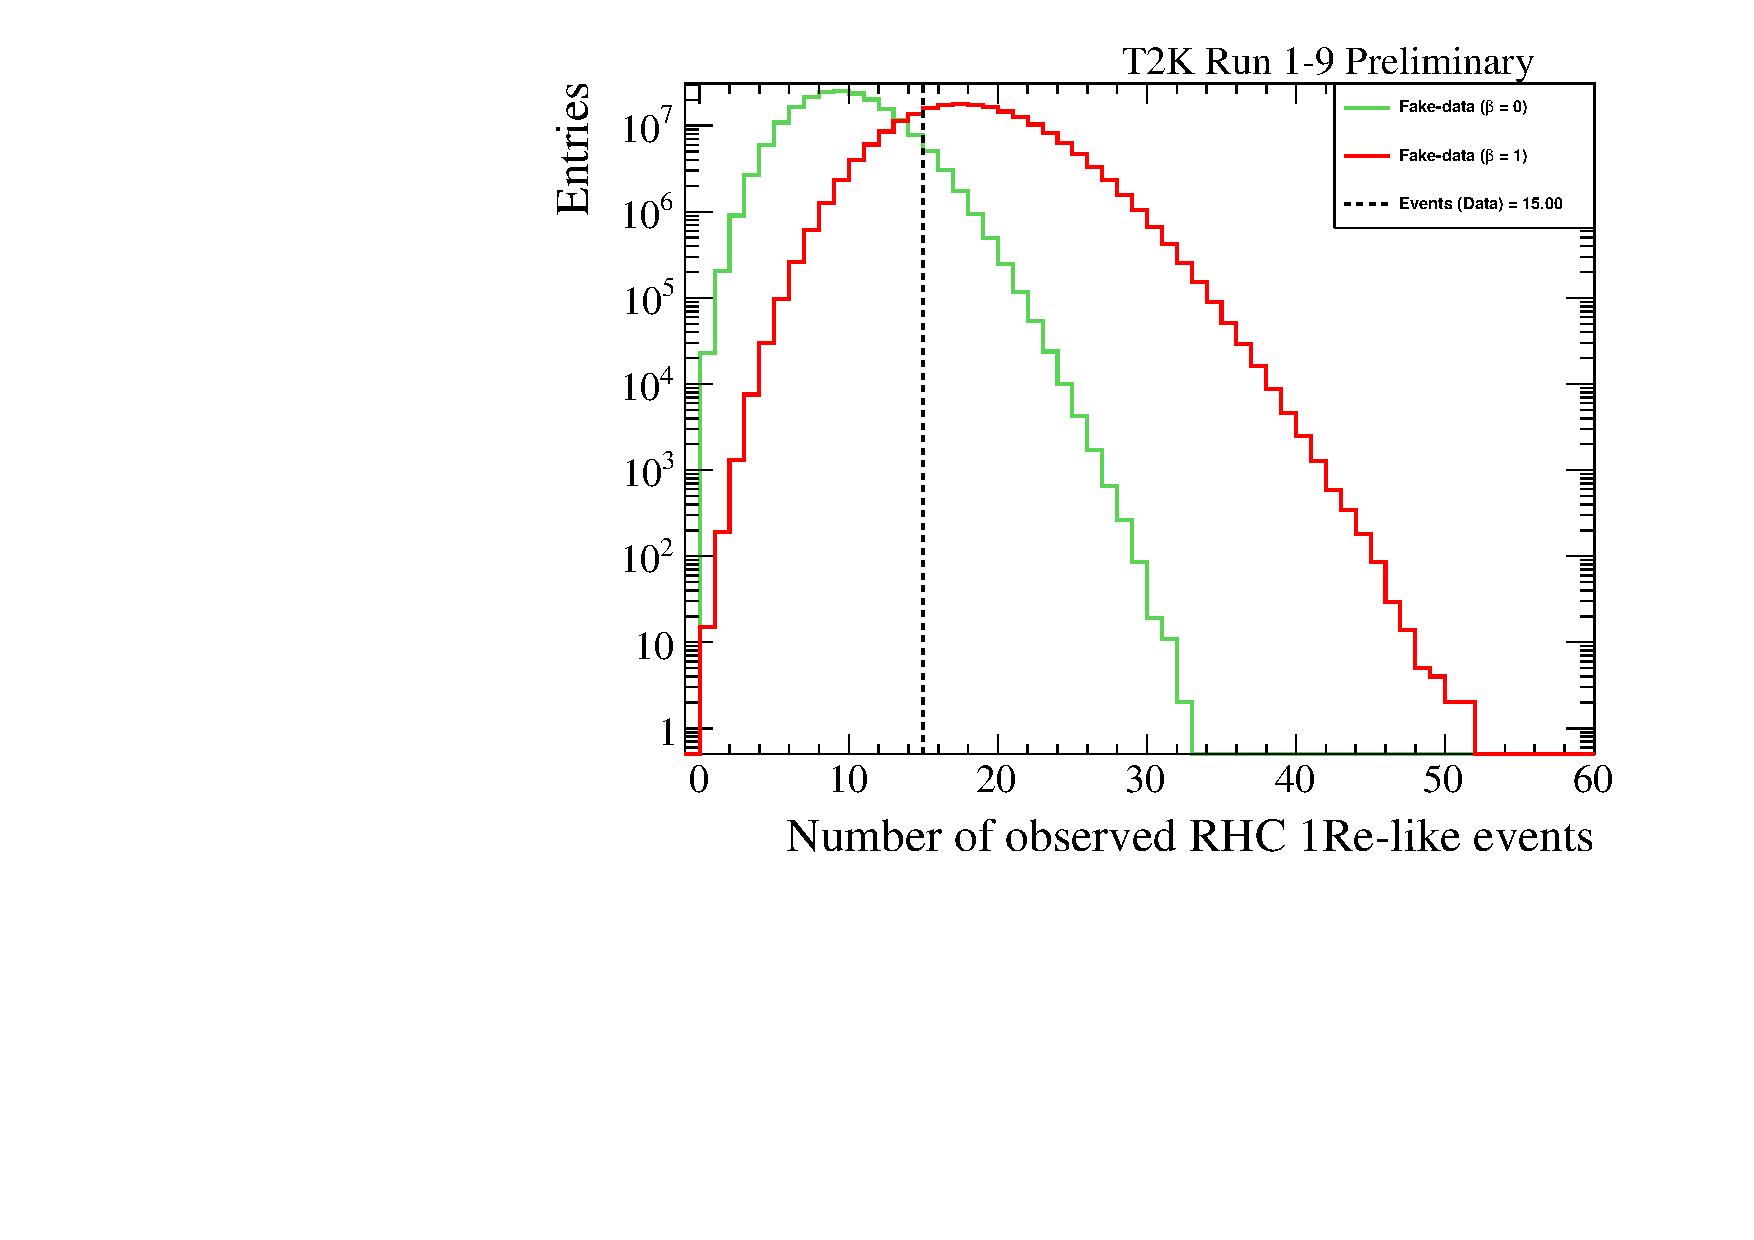
\includegraphics[scale=0.65]{data/Run1-9d/nuebarapp_graphs_nmargtoys=200k_nexp=20k_data_rate-only_MCsampling_VALOR_Nevents_logscale}
	\caption{The distribution of the total number of events in the antineutrino mode single-ring e-like sample from each of the \NToysFakeDataRateOnly\ toy experiments for both the $\beta = 0$ and $\beta = 1$ hypotheses. The distributions were produced using the method outlined in section \ref{sec:method_rate-only} using the Run 1-9d data spectra to calculate the likelihood. The dashed line corresponds to the total number of events given by the Run 1-9d data set.
	}
	\label{fig:data_rate-only_Run1-9d}
\end{figure}

\begin{figure}
	\centering
	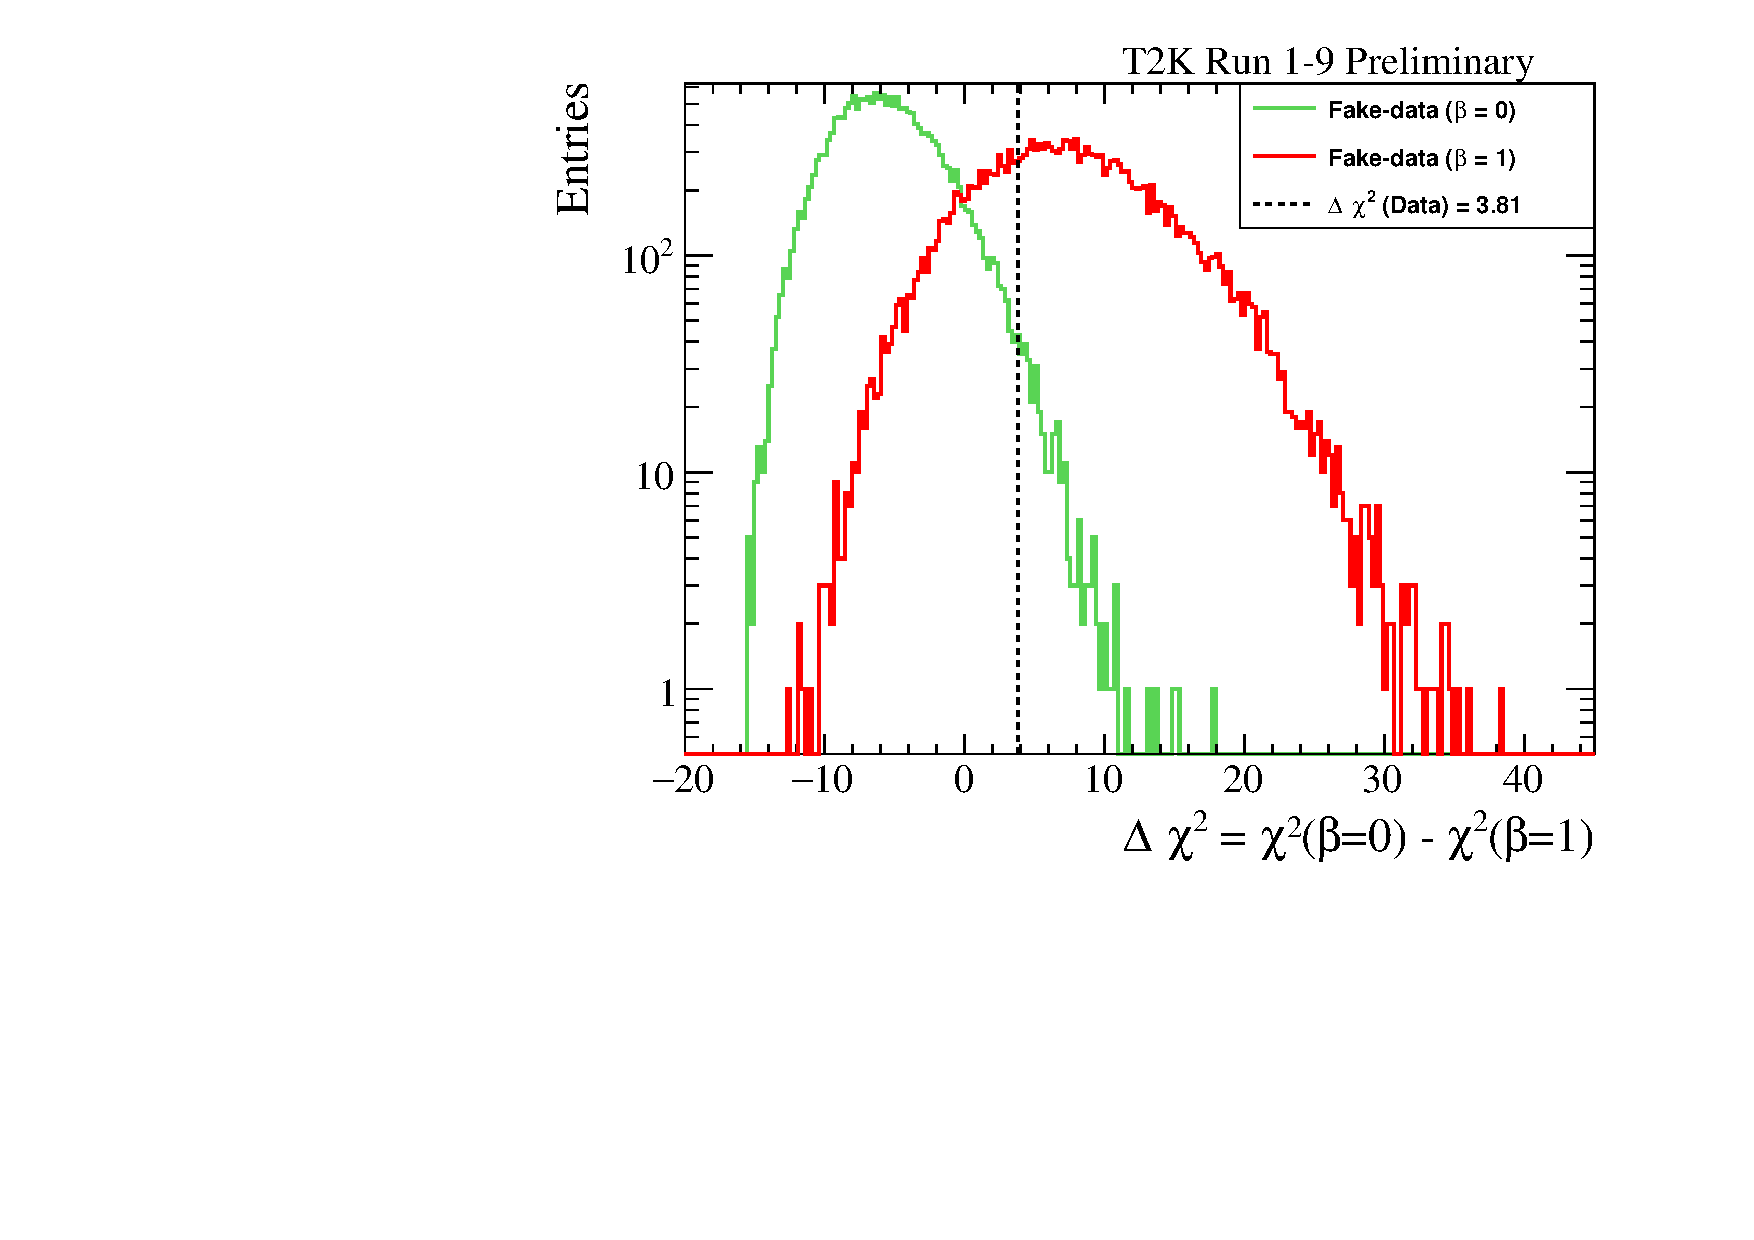
\includegraphics[scale=0.65]{data/Run1-9d/nuebarapp_graphs_nmargtoys=200k_nexp=20k_data_rate+shape_MCsampling_VALOR_Deltachisq_logscale}
	\caption{The distribution of $\Delta \chi^2$ values from each of the \NToysFakeDataRatePlusShape\ toy experiments for both the $\beta = 0$ and $\beta = 1$ hypotheses. The distributions were produced using the method outlined in section \ref{sec:method_rate+shape} using the Run 1-9d data spectra to calculate the likelihood. The dashed line corresponds to the $\Delta \chi^2$ value given by the Run 1-9d data set.
	}
	\label{fig:data_rate+shape_Run1-9d}
\end{figure}

\begin{table}
	\centering
	\begin{tabular}{|c|c|c|c|}
		\hline
		$\beta$				& Analysis		& p-value                		        & $\sigma$ 						           \\
		\hline
		\multirow{ 2}{*}{0} & rate-only		& \pvalRateOnlyBetaZeroDataRunOneNineD  & \sigmaRateOnlyBetaZeroDataRunOneNineD    \\
		\cline{2-4}
			   				& rate+shape	& \pvalRateShapeBetaZeroDataRunOneNineD & \sigmaRateShapeBetaZeroDataRunOneNineD   \\
		\hline
		\multirow{ 2}{*}{1} & rate-only		& \pvalRateOnlyBetaOneDataRunOneNineD   & \sigmaRateOnlyBetaOneDataRunOneNineD     \\
		\cline{2-4}
			   				& rate+shape	& \pvalRateShapeBetaOneDataRunOneNineD  & \sigmaRateShapeBetaOneDataRunOneNineD    \\
		\hline
	\end{tabular}
	\caption{Data p-values and event-rates for the $\beta = 0$ and $\beta = 1$ hypotheses using both the rate-only and rate+shape analyses and the full Run 1-9 dataset}
	\label{tab:data_pvals_R1-9d}
\end{table}


\begin{figure*}[htb]
	\center
	\begin{subfigure}[b]{0.49\textwidth}
		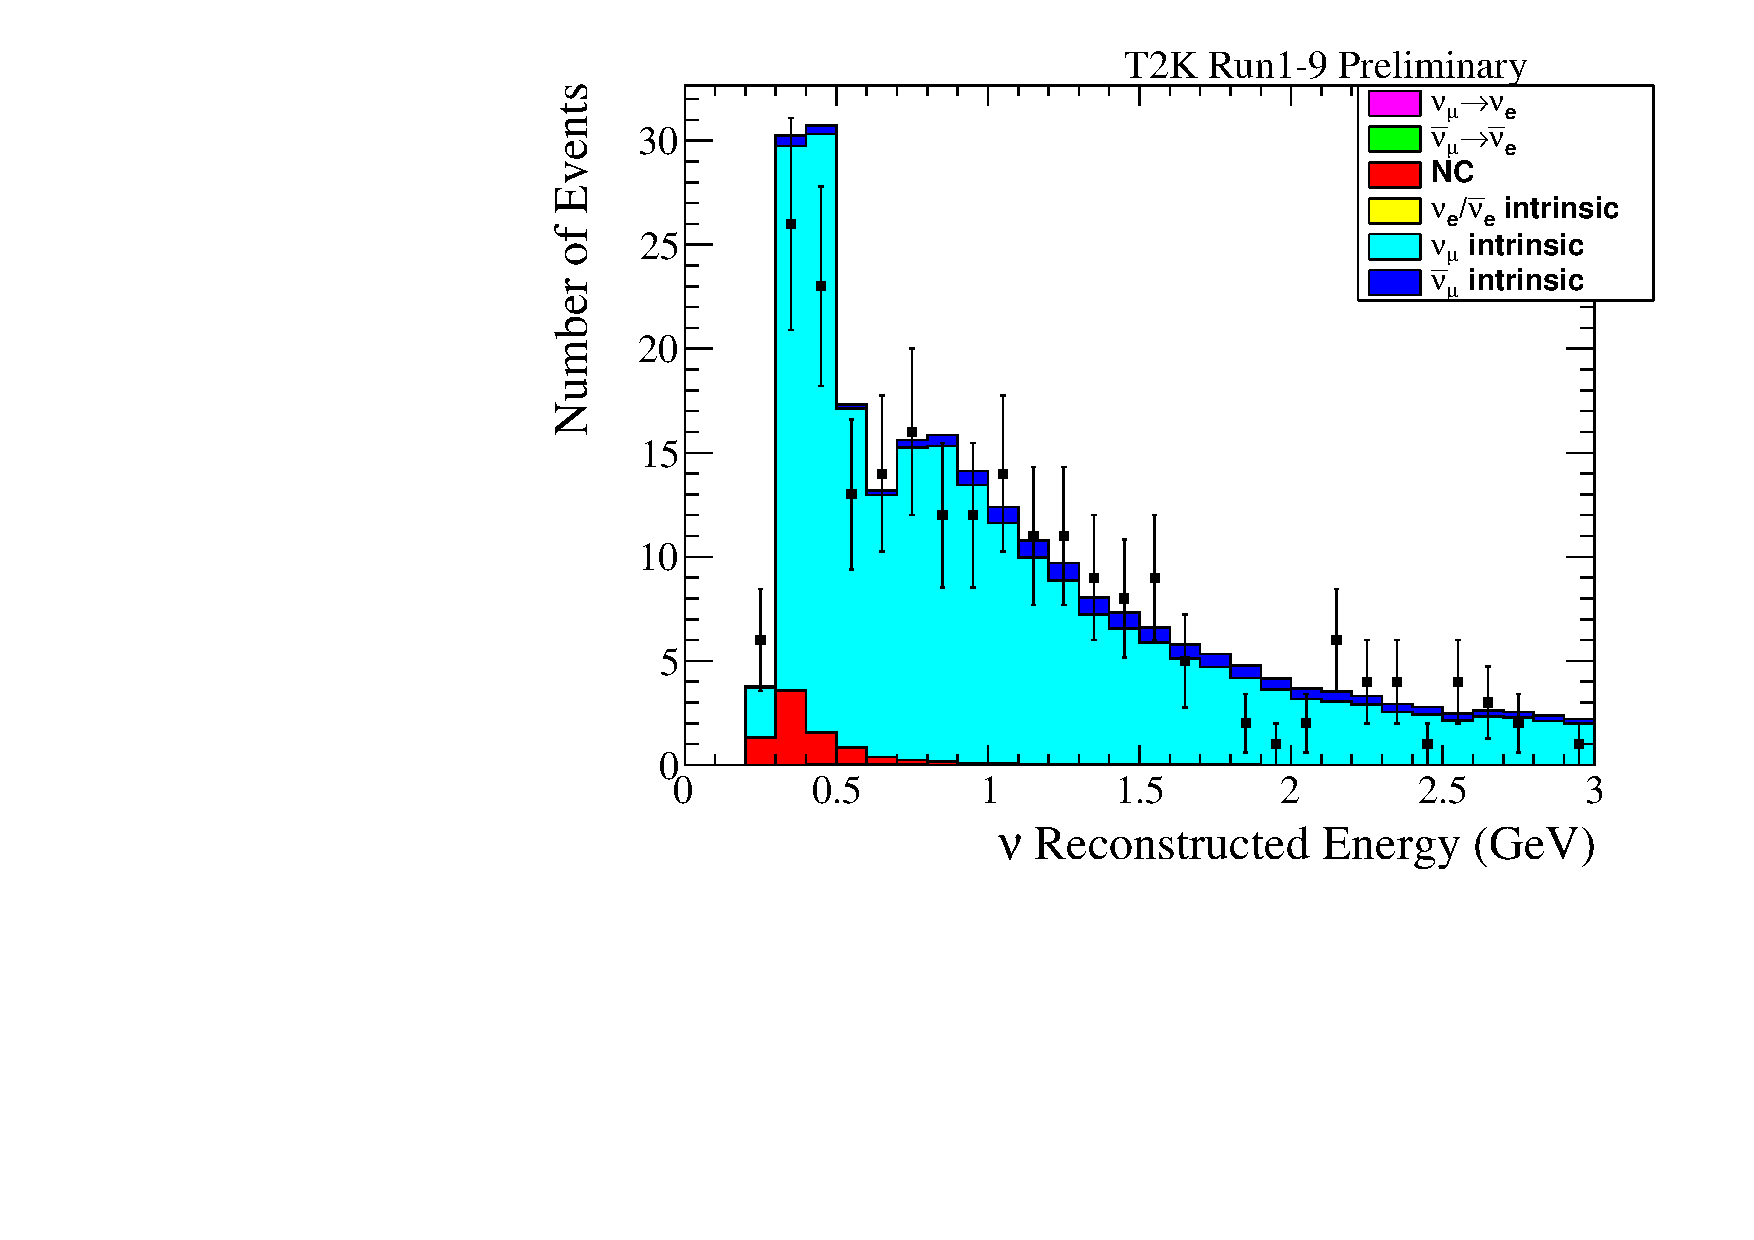
\includegraphics[width=0.9\textwidth]{spectra/Run1-9d/spectrum_AsimovA_1Rmu}
		\caption{Muon-like, neutrino mode}
	\end{subfigure}
	\begin{subfigure}[b]{0.49\textwidth}
		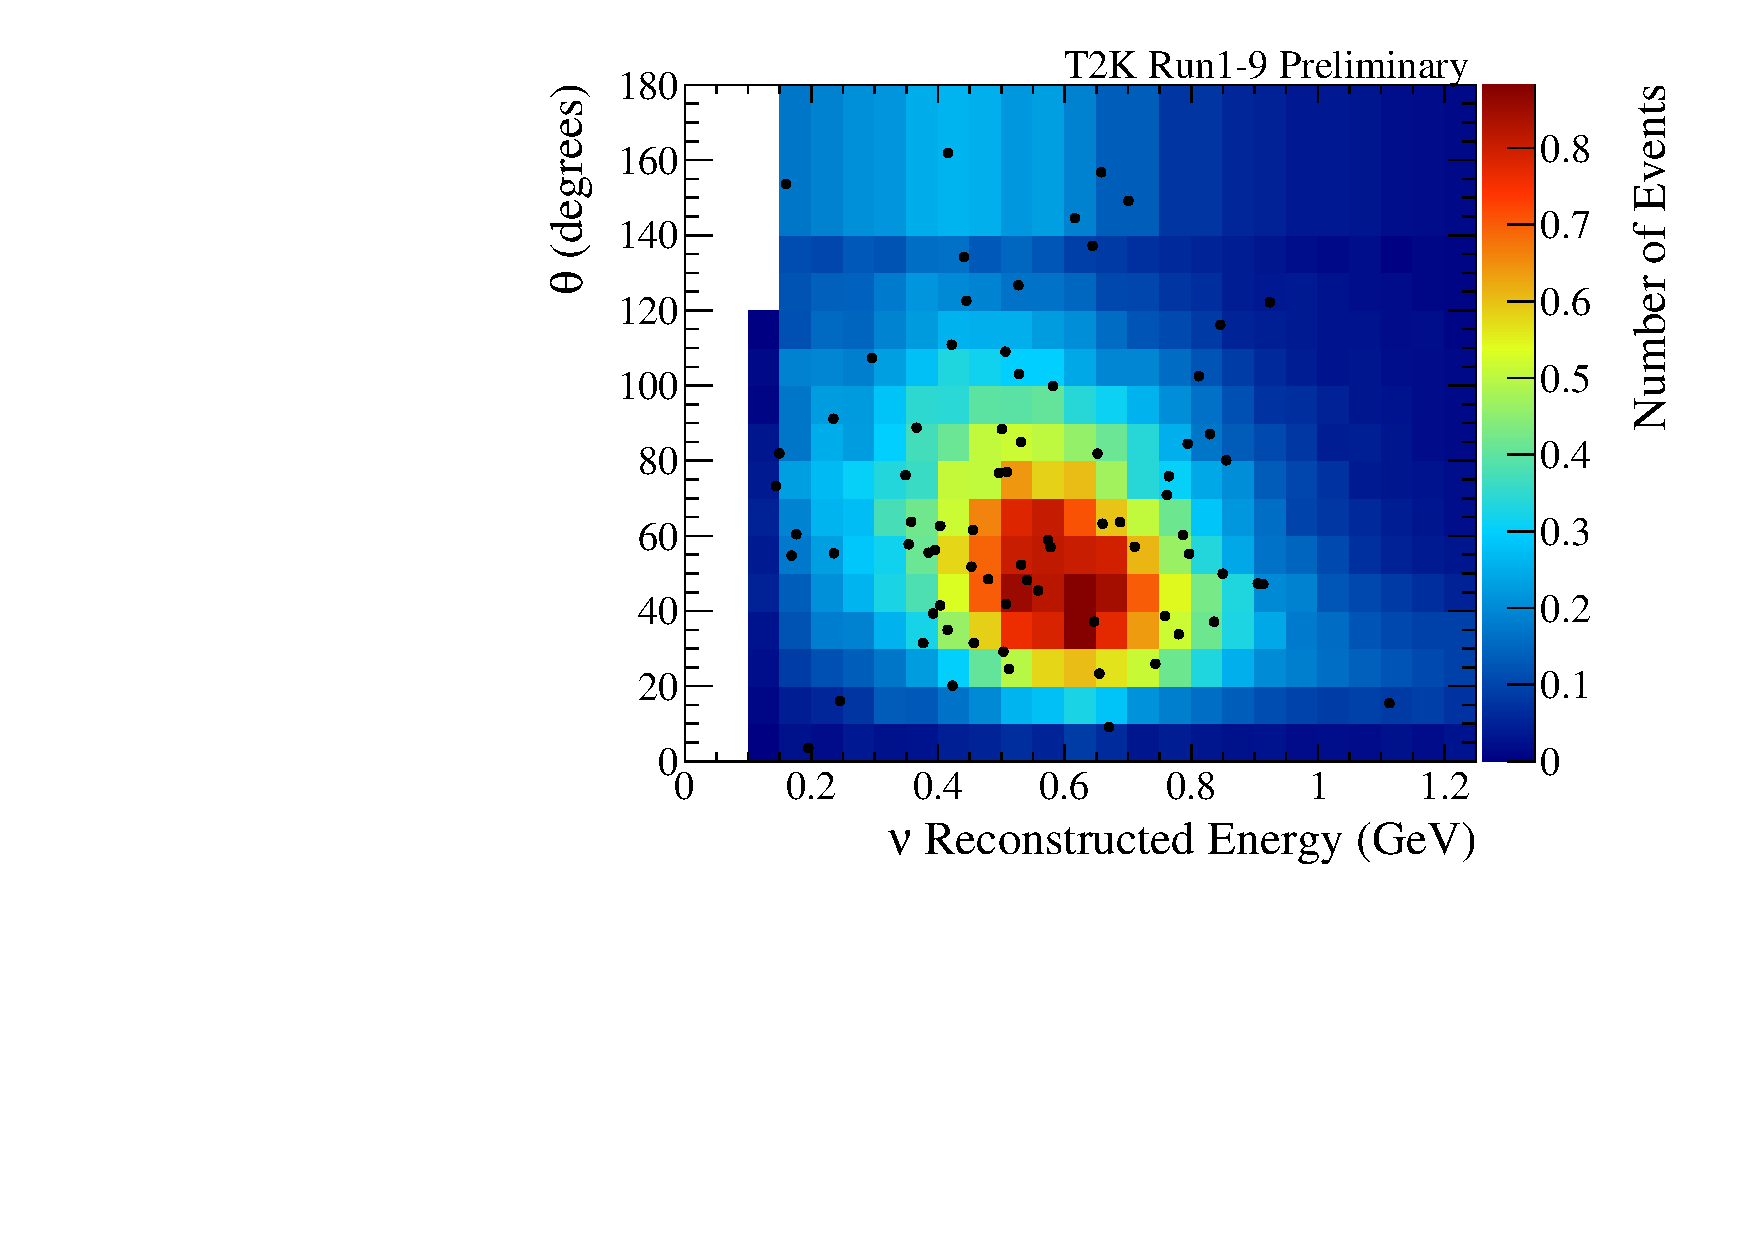
\includegraphics[width=0.9\textwidth]{spectra/Run1-9d/spectrum_AsimovA_1Re}
		\caption{Electron-like, neutrino mode}
	\end{subfigure}
	\begin{subfigure}[b]{0.49\textwidth}
		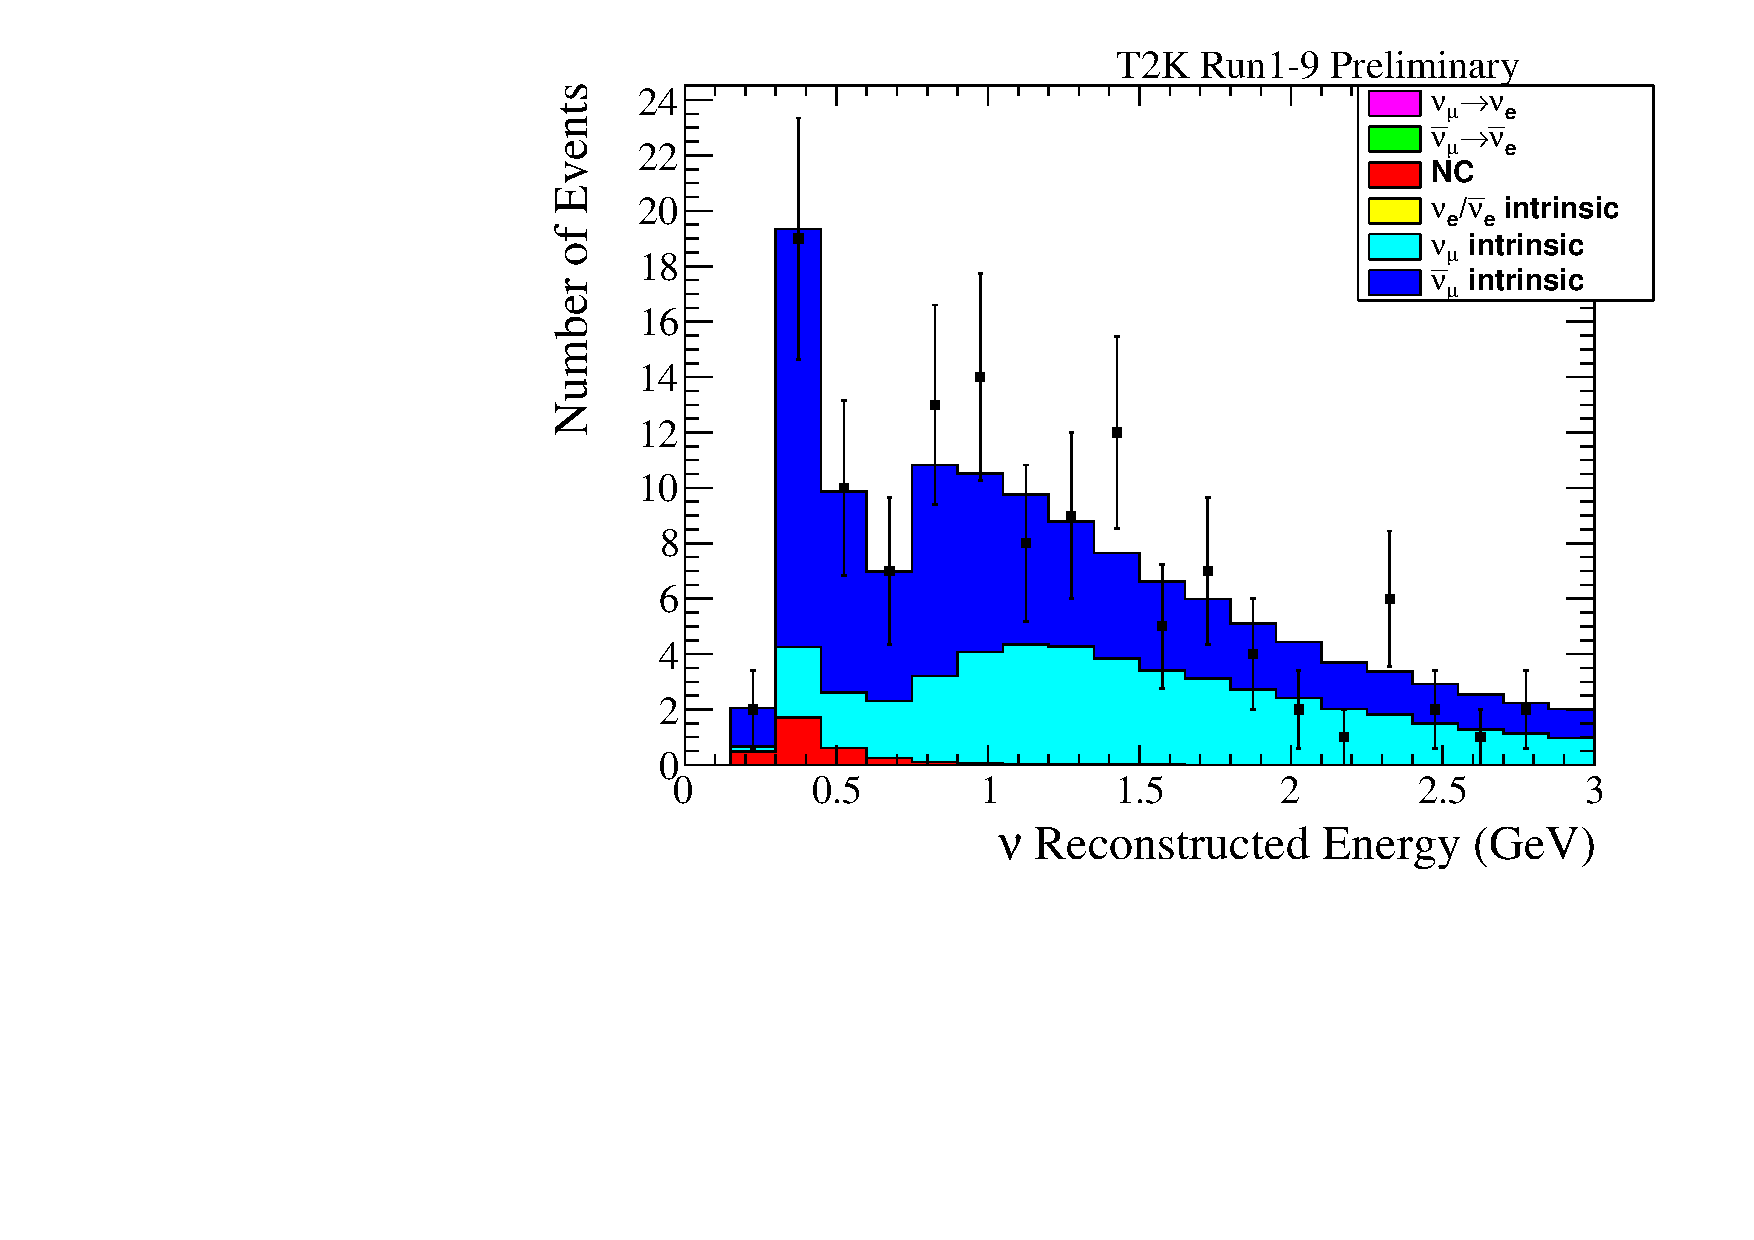
\includegraphics[width=0.9\textwidth]{spectra/Run1-9d/spectrum_AsimovA_RHC1Rmu}
		\caption{Muon-like, antineutrino mode}
	\end{subfigure}
	\begin{subfigure}[b]{0.49\textwidth}
		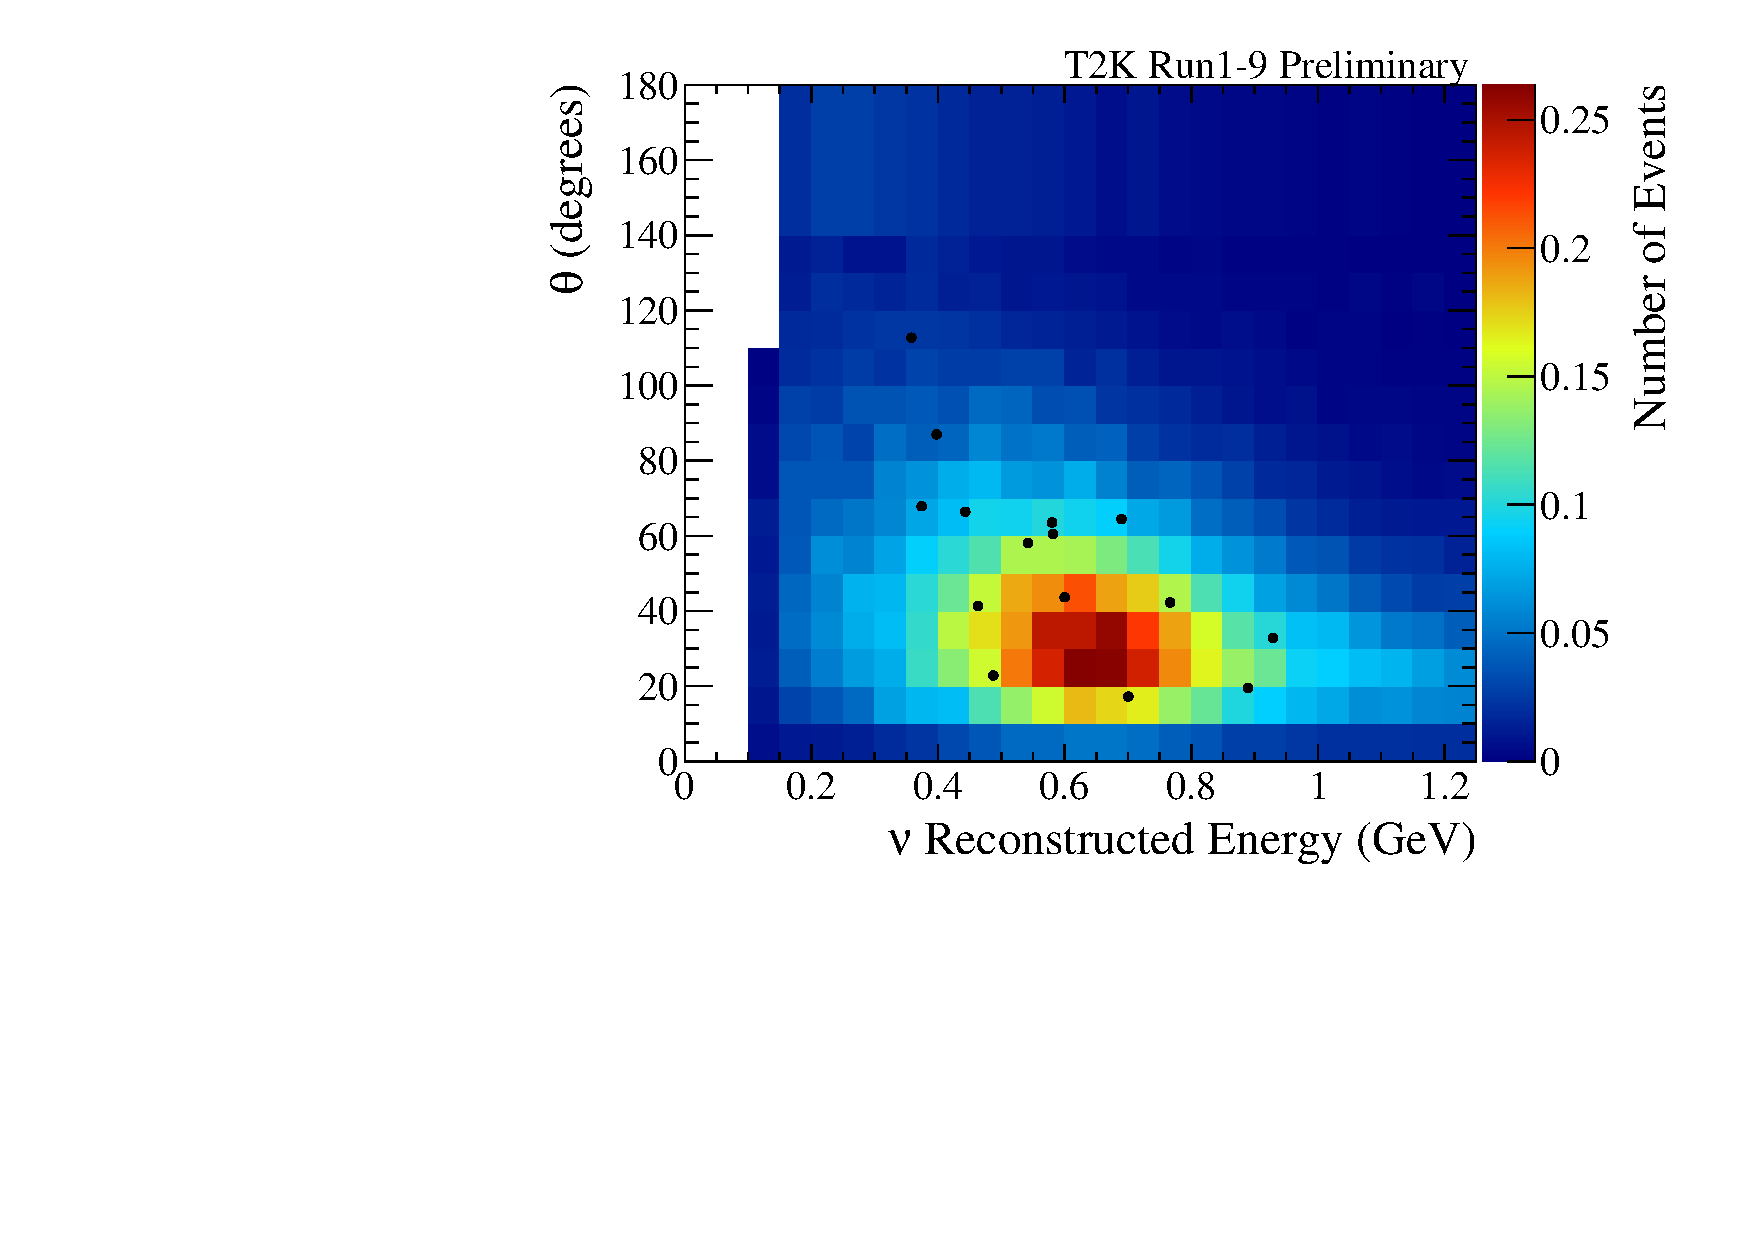
\includegraphics[width=0.9\textwidth]{spectra/Run1-9d/spectrum_AsimovA_RHC1Re}
		\caption{Electron-like antineutrino mode \label{fig:nuebar_tot_spectra_Run1-9d}}
		\label{fig:asimova_spectra_Run1-9d_RHC1Re}
	\end{subfigure}
	\begin{subfigure}[b]{0.49\textwidth}
		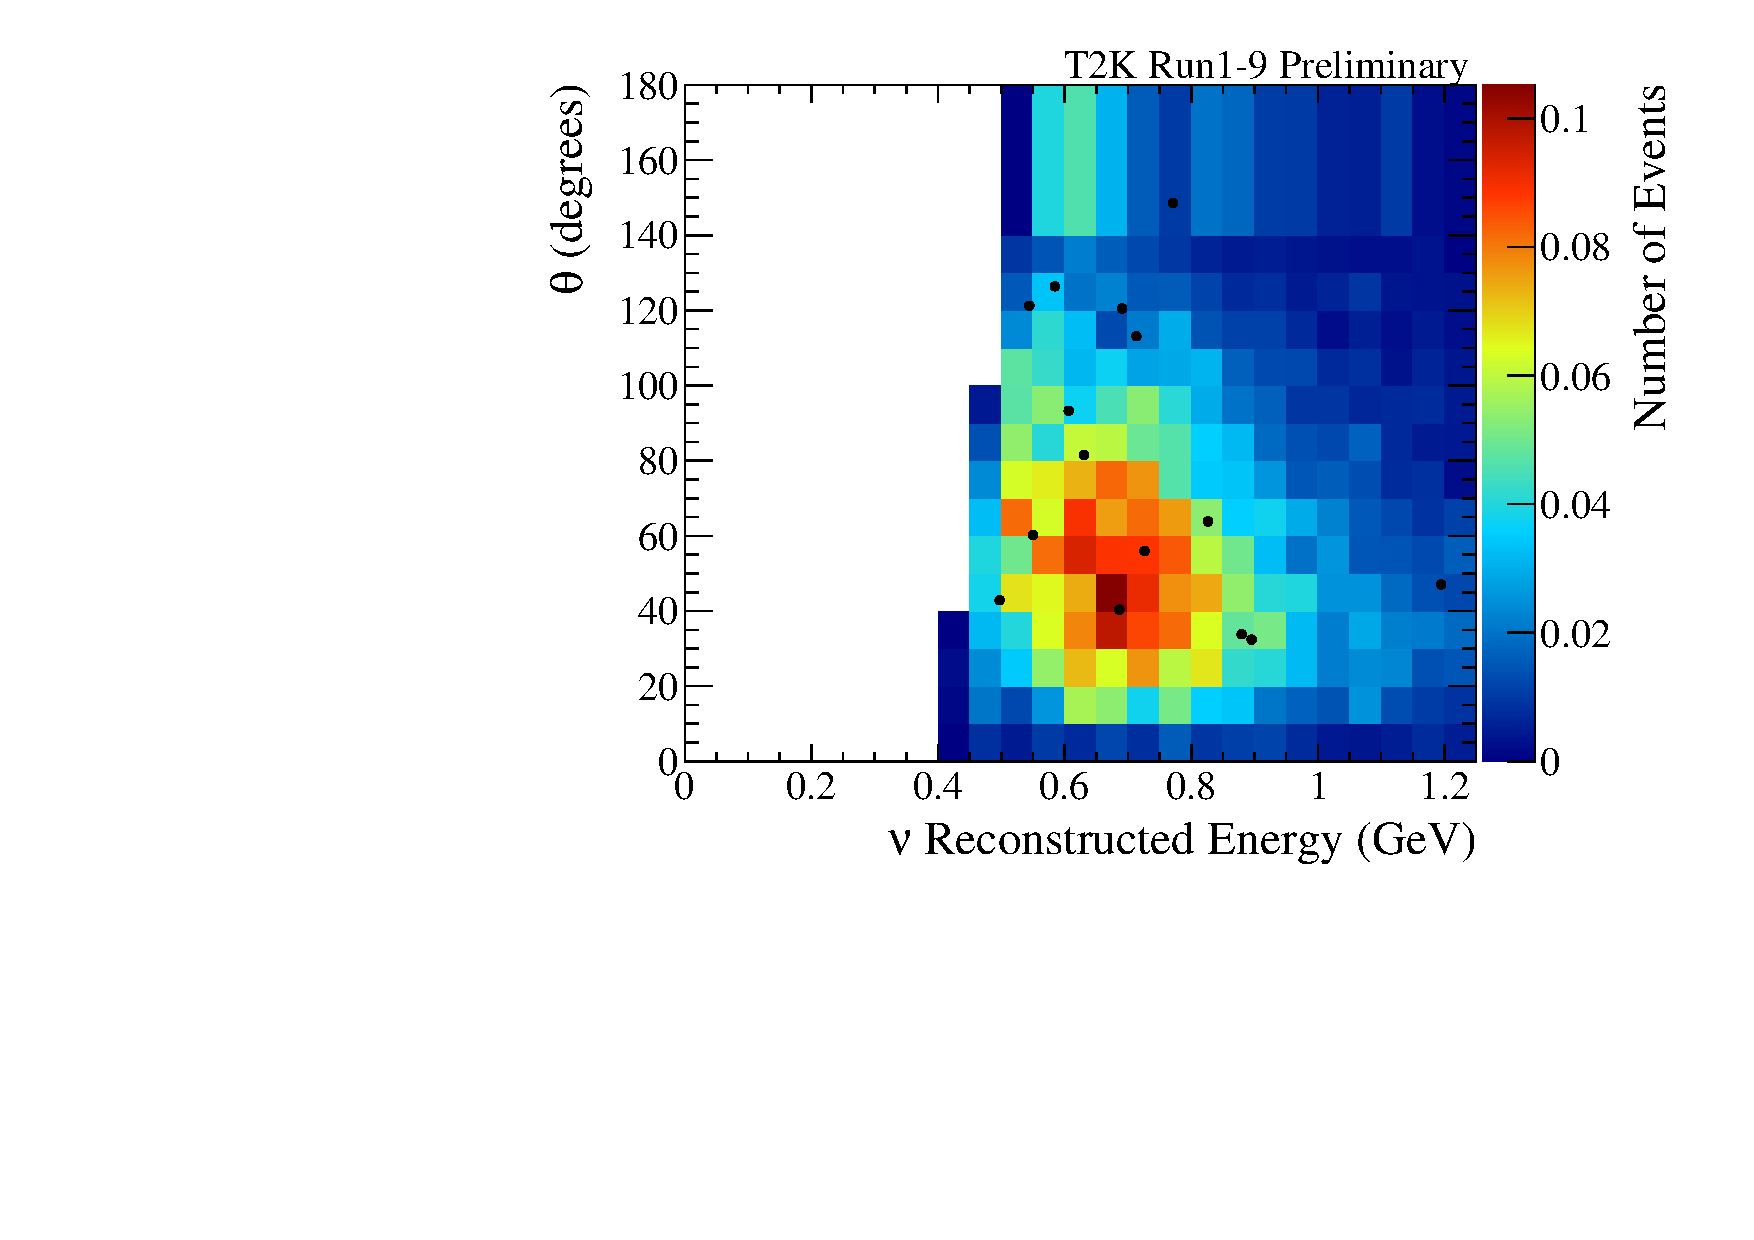
\includegraphics[width=0.9\textwidth]{spectra/Run1-9d/spectrum_AsimovA_MultiRe}
		\caption{\nueCConepi-like, neutrino mode}
	\end{subfigure}
	\caption {
		Predicted Asimov A spectra with Run 1-9 data superimposed. $\mu$-like distributions are a function of the reconstructed neutrino energy, while the $e$-like, including \nueCConepi, distributions are functions of both the reconstructed neutrino energy and the reconstructed angle between the outgoing lepton and the neutrino direction. The distributions correspond to the statistics collected in the full Run 1-9 data set. The spectra are generated with the oscillation parameters corresponding to the Asimov data set A shown in \cref{tab:osc_params_joint_asimovA}.
		%The spectra are generated with the systematic parameters described in \cref{sec:systematics} and the oscillation parameters corresponding to the Asimov data set A shown in \cref{tab:asimov_definition1}.
	}
	\label{fig:asimova_spectra_all_Run1-9d}
\end{figure*}
\clearpage

} % \colour{red}

